\documentclass{article}
\usepackage{tikz}
\usetikzlibrary{positioning}

\begin{document}

\begin{figure}[h]
    \centering
    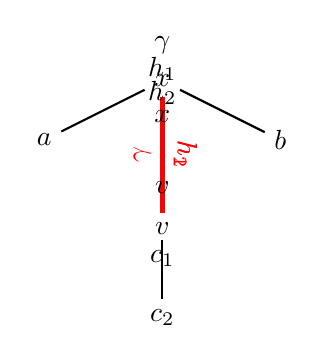
\begin{tikzpicture}[scale=1.5]
        % Define nodes
        \node (a) at (-1,0) {$a$};
        \node (b) at (1,0) {$b$};
        \node (c1) at (0,-1) {$c_1$};
        \node (c2) at (0,-1.5) {$c_2$};
        \node (v) at (0,-0.75) {$v$};
        \node (x) at (0,0.5) {$x$};
        
        % Draw edges
        \draw[thick] (a) -- (x);
        \draw[thick] (b) -- (x);
        \draw[thick] (c1) -- (v);
        \draw[thick] (c2) -- (v);
        \draw[thick] (x) -- (v);
        
        % Draw red edges and labels
        \draw[ultra thick, red] (x) -- node[above,sloped] {$h_1$} (v);
        \draw[ultra thick, red] (x) -- node[above,sloped] {$h_2$} (v);
        \draw[ultra thick, red] (v) -- node[above,sloped] {$\gamma$} (x);
        
        % Label the vertices
        \node at (0,0.8) {$\gamma$};
        \node at (0,-0.4) {$v$};
        \node at (0,0.6) {$h_1$};
        \node at (0,0.4) {$h_2$};
        \node at (0,0.2) {$x$};
    \end{tikzpicture}
    \caption{Figure for the proof of \cref{prop:3-cyc11}, case \eqref{case:2}. A $3_2$-cycle quartet network with internal cut edge contracted to length 0, other edge probabilities $h_1, h_2, x$, and hybridization parameter $\gamma$.}
    \label{fig:3-cyc11-case2}
\end{figure}

\end{document}